\chapter{Android系统 }  
\label{chp:background}


本章首先会简要介绍Android系统架构,其次会对Android中的Activity组件做基本介绍,接着会着重介绍Android中常见的两种多线程交互方式,最后将指出本文系统在实现上的难点。

\section{Android系统架构}

Android是基于Linux内核开发的的开源操作系统,隶属于Google公司,主要用于触屏移动设备如智能手机、平板电脑与其他便携式设备,是目前世界上最流行的移动终端操作系统之一。


在系统架构上,Android自下到上,可以分为四层:Kernel层、Library和Android Runtime(Dalvik/ART)、Framework、Application等,如~\autoref{fig:Android-Framework}所示。
Kernel层是硬件和软件层之间的抽象层,主要是设备的驱动程序,例如:显示驱动、音频驱动、蓝牙驱动、Binder IPC驱动等。
Library和Android Runtime(Dalvik/ART): Library,顾名思义就是向上层提供各种这样的基础功能,例如SQLite数据库引擎,Surface Manager显示系统管理库。
Android Runtime主要是运行Android程序的虚拟机\eat{,在不同版本的系统上对应着不同的虚拟机,例如在Android 5.0及以上是ART,而在Android 4.3及以下是Dalvik,而Android 4.4两者都有}。
Framework层主要是系统管理类库,包括Activity的管理,消息通知的管理;同时,它是Application的基础架构,为应用程序层的开发者提供了API,其存在简化了程序的开发。
而Application就是我们平时接触的应用,开发人员公国调用底层Framework提供的API实现相应的接口。

虽然Android应用程序是使用Java语言开发的,但是它和传统的Java程序有着很大的不同,具体有如下几点:

\begin{figure*}[!h]
	\centering
	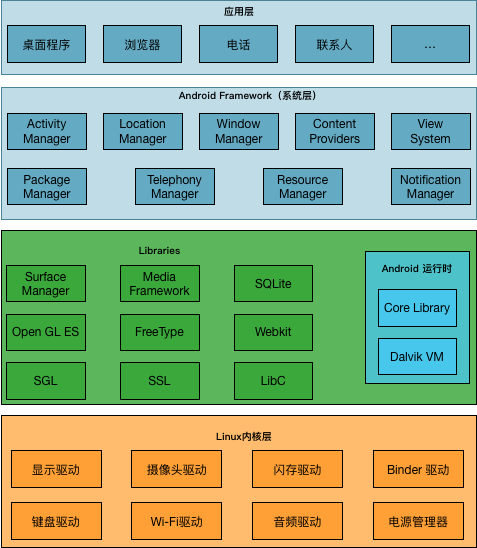
\includegraphics[width=0.8\textwidth]{./Figures/Android-Framework.png}
	\caption{Android系统框架图}
	\label{fig:Android-Framework}
\end{figure*}


\textbf{基于事件驱动的系统架构:}
在设计上,Android应用程序的系统架构为事件驱动架构。在开发过程中,没有传统程序中入口函数Entry Point的概念。
应用程序中通用的业务逻辑(例如应用程序如何启动退出、应用的窗口如何创建销毁等)存在于Android Framework中。
%这也使得Android应用程序的分发文件(即APK文件)相对较小。

\textbf{面向组件的编程模式:}
Android程序中较为常见的是组件(例如Activity、Service、Content Provider、Broadcast Receiver),它是应用程序运行的最小单元,受到Android Framework的直接调度。
开发人员通过继承这些组件,重写对应的生命周期函数,实现对应的业务需求\eat{(界面的布局、页面状态的保存等)},而这些组件的生命周期由Framework直接调度完成。

\textbf{逻辑实现依赖于回调函数和多线程通信:}
由于Android应用程序采用的是基于单线程消息队列的事件驱动架构,因此,界面相关的操作只允许出现在主线程(UI Thread)中,耗时操作只能在工作线程(Worker Thread)中进行。
通常的,开发人员往往会借助回调函数处理控件的响应事件,利用多线程交互串联界面相关操作和耗时操作,完成对应的业务。


\section{Android中的Activity组件}



在Android应用程序运行过程中,Activity向用户展示图形界面,响应用户的反馈,和其他组件一同完成相关业务,扮演着最为重要的角色。%\cite{Activity2:online}。
由于Android应用程序在架构选型上采用了事件驱动模型,为了便于协调应用内部状态的管理,Android组件通常有生命周期的概念,Activity也不例外。
Android系统将Activity的运行状态分为以下四种,Activity的生命周期就是Activity在这些状态之间的跳转。



\begin{itemize}
		\setlength{\itemsep}{-5pt}
		
	\item 运行态:在该状态下, Activity处于页面最前端时,用户可以与Activity进行交互。
	一般的,用户可见并可以进行交互的Activity均处于这个状态。
	
	\item 暂停态:在该状态,Activity仍然可见,但是失去了窗口的焦点。
	当一个Activity之上出现非全屏的窗体(例如对话框)但未被完全遮挡时,Activity就处于这个状态。
	处于暂停状态的Activity仍处于存活状态,保存着所有的内存数据。%,只有当系统内存极度紧张时,才有可能被系统杀死回收。

	\item 停止态:当一个Activity被其他的Activity完全遮挡时,处于这个状态。
	处于该状态的Activity仍然可以保留所有的内存数据,只是对用户不可见。
	系统在需要内存的情况下,可以采用相应的策略对Activity进行杀死回收操作。
	
	\item 终止态:当用户自动退出Activity时,Activity将进入该状态;当Activity处于暂停态或者停止态时,系统由于内存原因可能会将上述两种Activity杀死回收。
\end{itemize}



\begin{figure*}[!ht]
	\centering
%	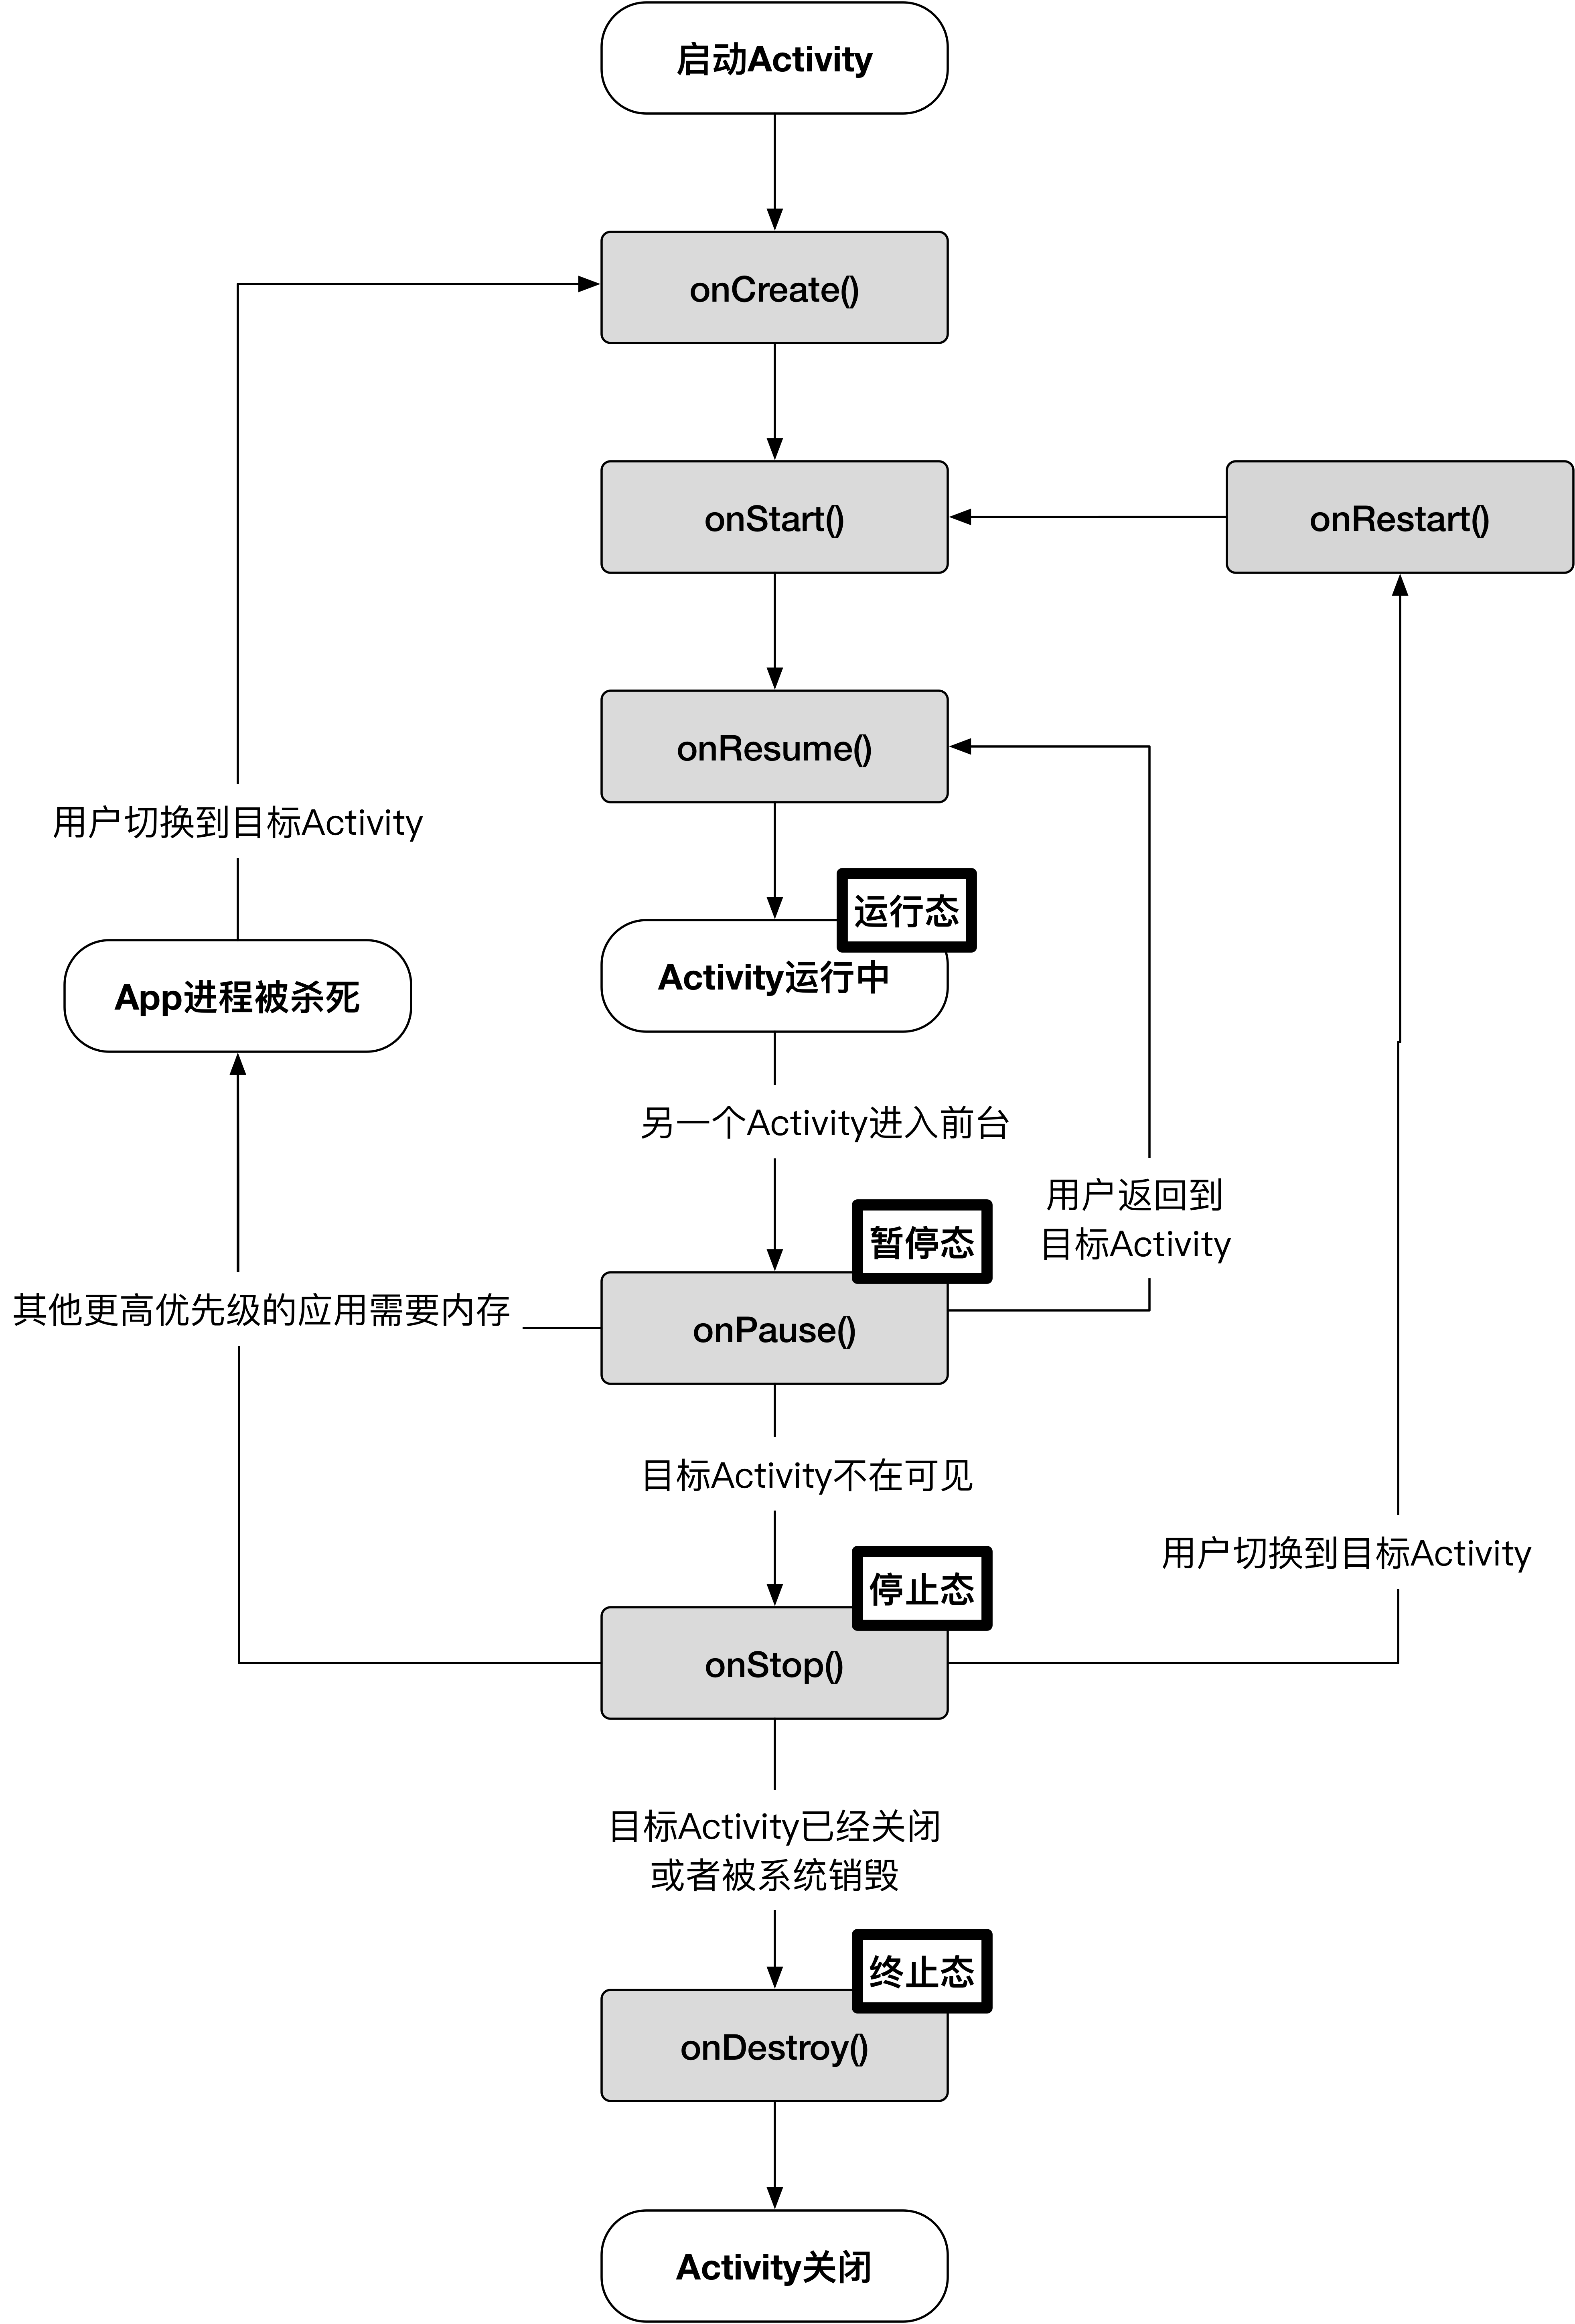
\includegraphics[width=0.9\textwidth]{./Figures/Activity-lifecycle.png}
	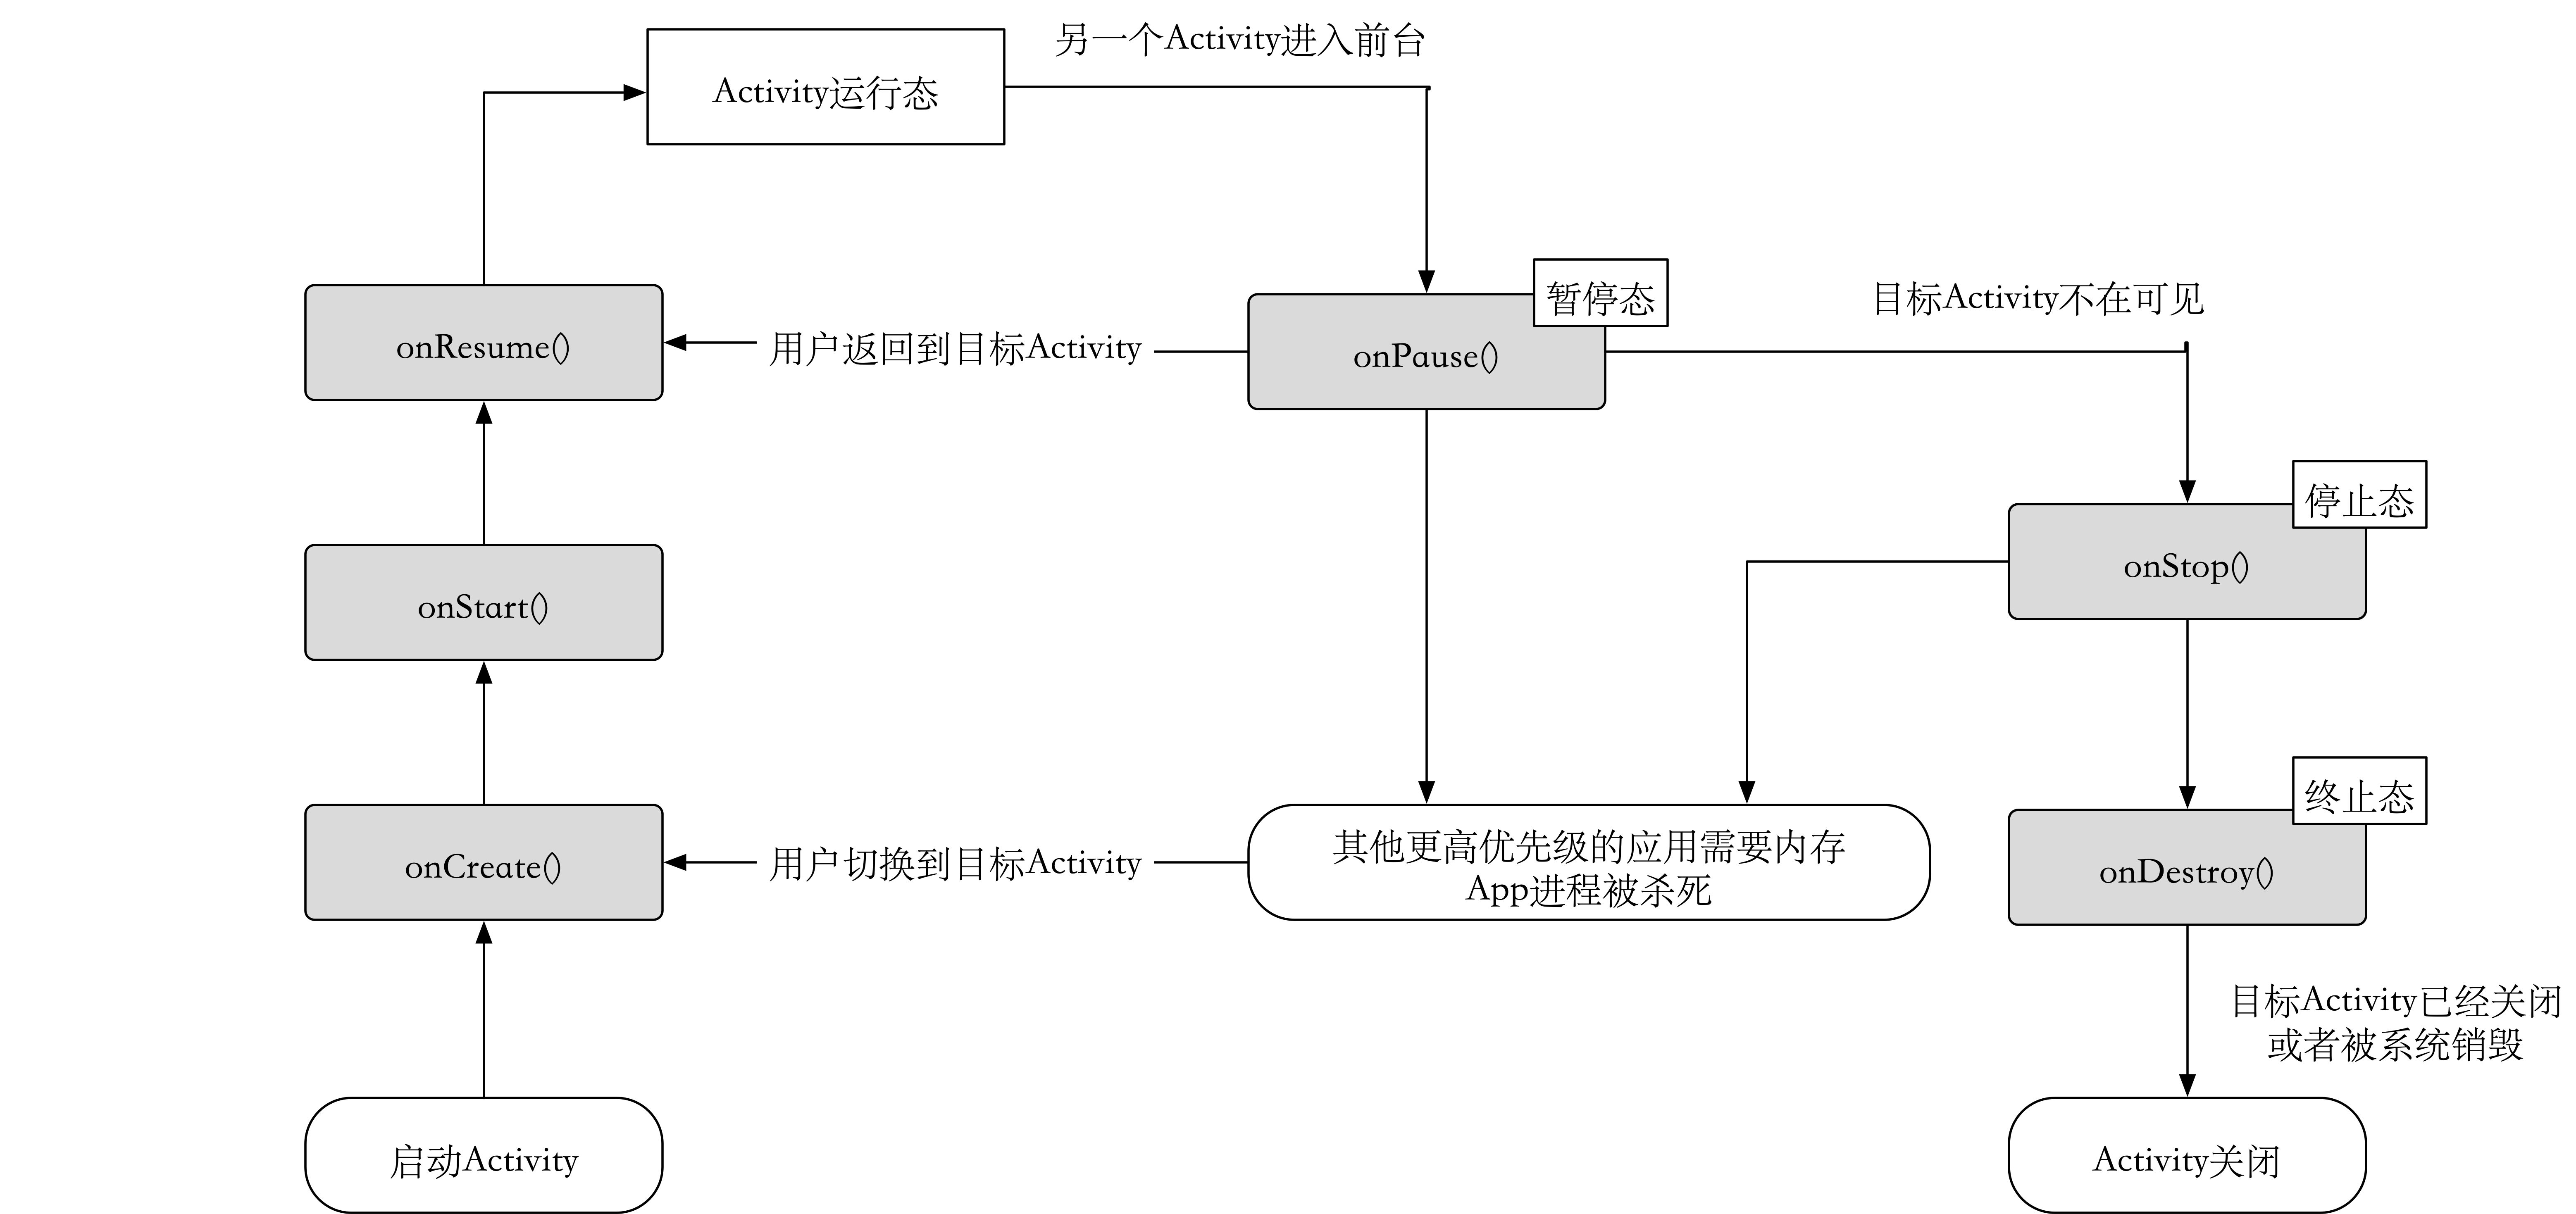
\includegraphics[width=0.9\textwidth]{./Figures/Activity-lifecycle-Landscape.png}
	
	\caption{Activity的生命周期}
	\label{fig:Activity-lifecycle}
\end{figure*}

Activity的生命周期受到Activity在运行时的内存分布、环境状态以及业务逻辑的影响,由Android系统直接负责调度。
和\code{Activity}生命周期相关的方法包括\code{onCreate()}、 \code{onStart()}、\code{ onResume()}、 \code{onPaused()}、 \code{ onStop()}和\code{onDestroy()}等,方便开发人员在\code{Activity}的状态发生变化时对程序的运行时数据和应用状态做适当的处理操作。
\code{Activity}的生命周期如\autoref{fig:Activity-lifecycle}所示:



当用户点击应用图标,系统启动应用程序后,系统会创建、启动Activity并使之可以和用户进行交互。
在这个过程中,\code{onCreate()}、\code{onStart()}、\code{onResume()}等方法被回调,Activity最终处于运行态;


当Activity被其他窗体遮挡,只失去焦点,仍处于可见状态时,Activity的状态从运行态变成暂停态,\code{onPause()}方法会被回调;当Activity重新获得焦点时,\code{onResume()}方法会被调用;

当Activity切换到另一个Activity时,原来Activity将从运行态变为停止态,\code{onPause()}、\code{onStop()}等方法会被调用;
当返回原来的Activity时,\code{onStart()}、\code{onResume()}等方法会被调用,Activity从暂停态变为运行态。
%将从从运行态变成暂停态时,Activity只失去焦点,仍处于可见状态,\code{onPause()}方法会被回调;当Activity重新获得焦点时,\code{onResume()}方法会被调用;

当用户点击“返回键”返回到桌面时,Activity会失去焦点,在用户的视野中消失,直至被系统回收,
对应的状态也从运行态经暂停态、停止态,变为终止态,期间\code{onPause()}、\code{onStop()}、\code{onDestroy()}等方法被回调。

\eat{
当用户从一个界面回到原来的界面时,原来的Activity从停止态重启,出现在设备界面上,获得交互焦点,
\code{onStart()}、\code{onResume()}等方法被回调;
}


\section{Android中的多线程交互}
Android系统在架构设计上采用了事件驱动架构。在多线程并发访问时,若UI控件对于各线程均是可见的,并发对控件做读写操作会使控件处于不可预期的状态;
若贸然对控件使用锁机制,访问控件的各个线程之间存在竞争关系,阻塞相关线程业务逻辑的执行,使得应用变得复杂低效。
%上述情况对于应用程序都是不可接受的。
为了避免此类低效率问题,Android系统在设计事件驱动架构时,采用了单线程的消息队列,即只允许在主线程(也称为Ui线程)进行界面更新操作,不允许在其他线程(也称为工作线程)进行界面更新操作。
另外,为了保证应用程序界面渲染和事件响应的及时性,任何在主线程上产生的耗时操作(例如加载磁盘上的图片、网络请求等)都是不被允许的。
换而言之,当应用程序需要进行耗时操作时,这个操作往往会在一个新的线程中执行,而不是在主线程中。


Android系统架构中的单线程消息队列以及主线程的非阻塞性,使得界面更新和耗时操作分散在不同的线程中。
只因如此,多线程交互在Android应用程序开发过程中十分常见。
从整体上,系统提供的交互方式分为两种:基于Java的多线程交互和基于Handler的交互方式。%\cite{androidSourceCode}。

\subsection{基于Java的多线程交互}

Android应用程序是在Java的基础上开发的,因此,开发人员可以采用和Java应用相同的调用方式启动工作线程,并在对应的线程上完成业务逻辑。
但是,Java API只能实现业务逻辑从原有线程转移到新的工作线程上,不能重新返回到主线程上。
为此,Android系统在Java API的基础上还提供了API \code{void runOnUiThread (Runnable runnable) }。
该API可以帮助开发人员将业务逻辑的执行从工作线程转移到主线程上,该API也符合Android只允许在主线程上更新界面这一基本设计原则。
但是,该API也存在着一些弊端,例如\code{runOnUiThread(Runnable)} API的定义位于类\code{android.app.Activity}。
这也就意味着,当业务逻辑的上下文脱离了Activity这一组件,将无法通过该API将业务逻辑转移回主线程,
同时基于接口的函数参数定义方式对于跨线程的参数传递也不是十分友好。
为此,Android提供了基于Handler的多线程交互方式。

\subsection{基于Handler的多线程消息调度}

为了满足开发人员多样化的业务在多线程间的切换,Android提供了基于Handler消息调度的多线程交互方式。



\begin{figure*}[h]
	\centering
	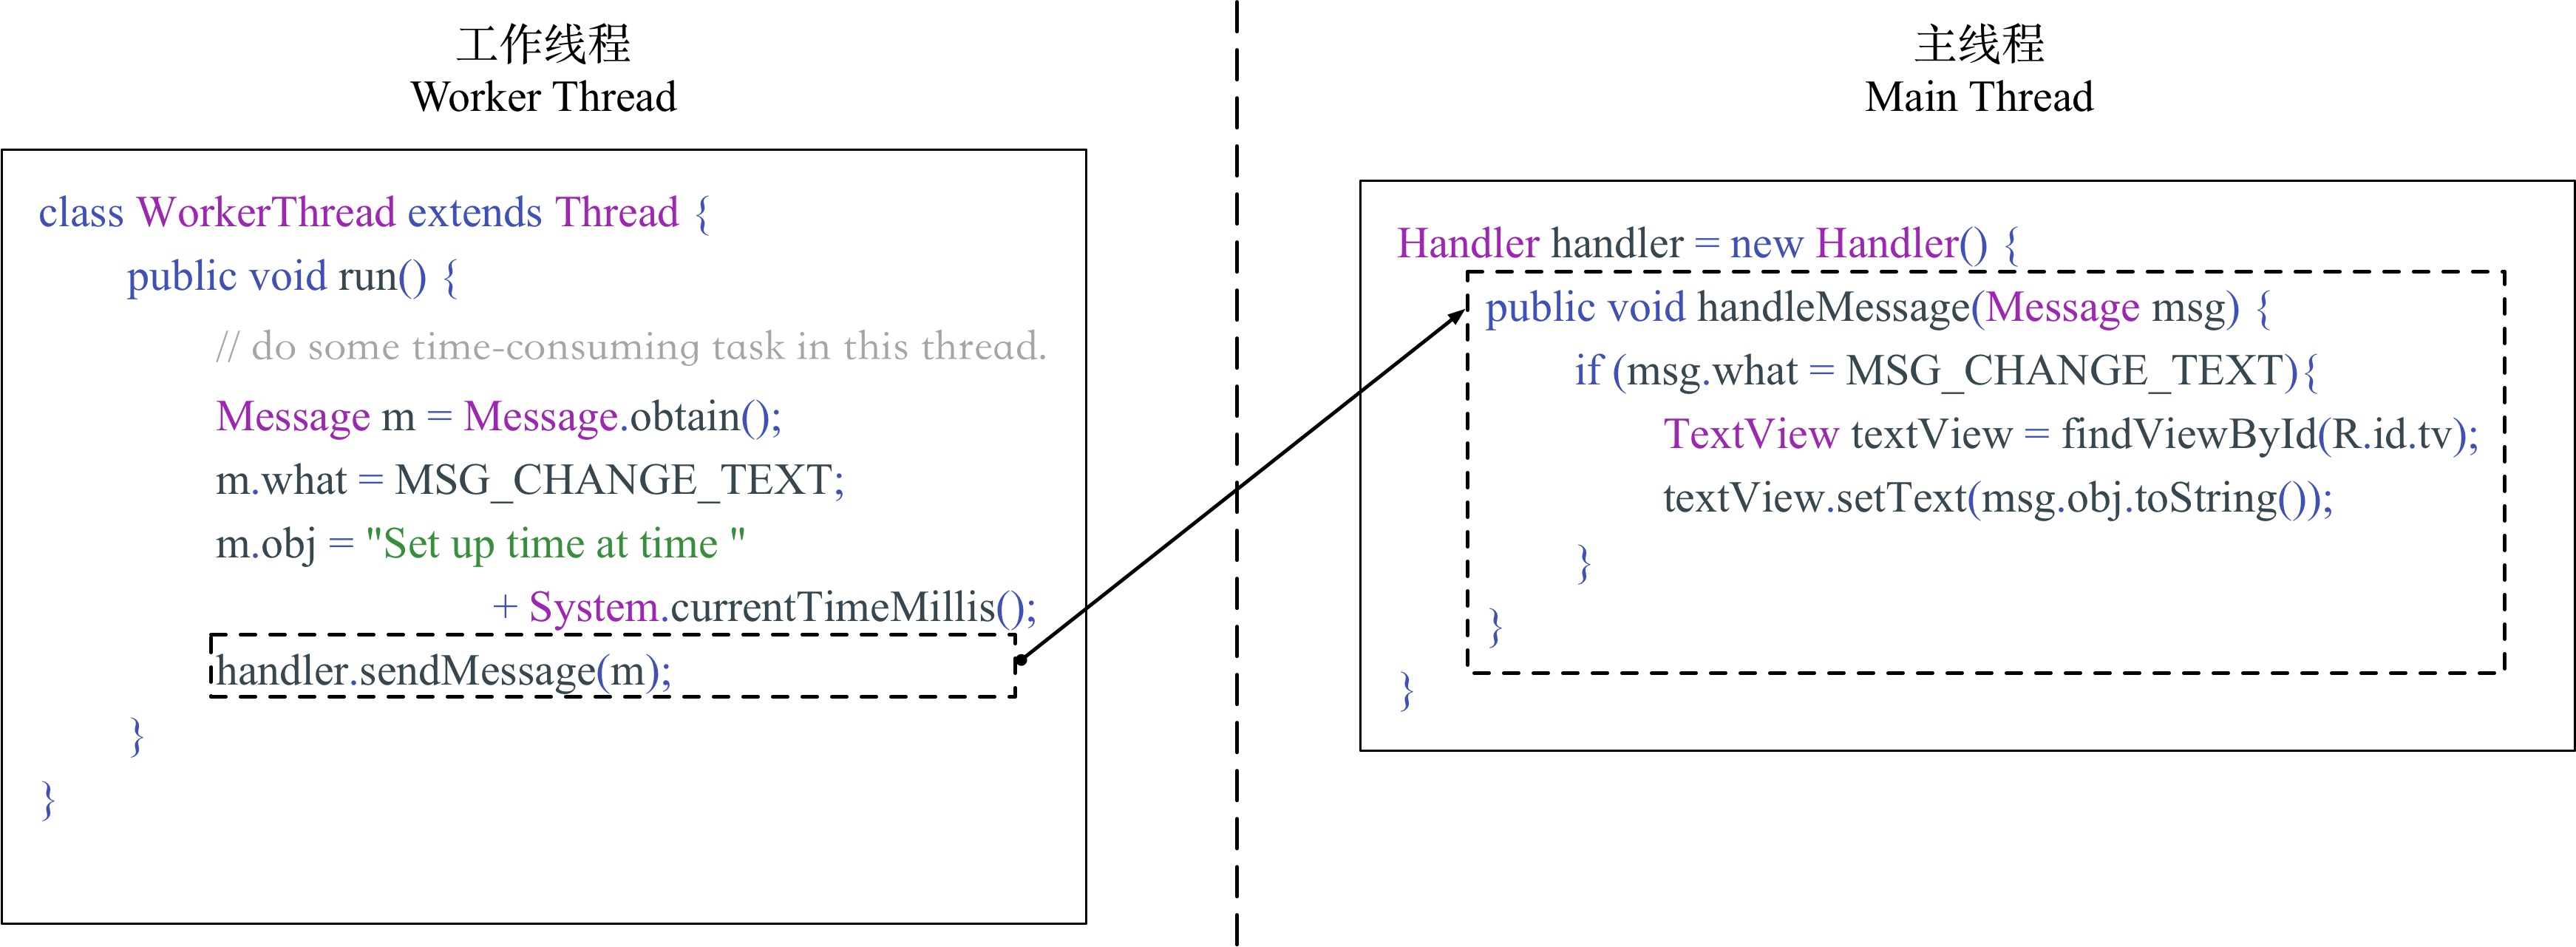
\includegraphics[width=0.9\textwidth]{./Figures/handler-code.png}
	\caption{Handler的使用实例}
	\label{fig:handler-code}
\end{figure*}


\autoref{fig:handler-code}为关于Handler的使用示例。
图中对应的场景为应用由于业务需要获取一个字符串,并将这个字符串展现在用户界面上。
考虑到获取字符串的过程比较耗时,可能会阻塞主线程的相关业务,因此我们会在工作线程执行这部分逻辑(如\autoref{fig:handler-code}-左所示),而在主线程执行信息展现的逻辑(如\autoref{fig:handler-code}-右所示)。
具体的,在工作线程中,用户生成的字符串和对应的逻辑代码\code{MSG\_CHANGE\_TEXT}封装到\code{Message}对象中,通过Handler发送出去;
Handler在主线程中收到了该\code{Message}对象时,会根据逻辑代码(即\code{Message.what}的值)决定进行对应的逻辑处理(本例中,对应逻辑为更新界面信息)。


%用户在工作线程执行生成一个字符串,将生成的字符串传递给Message对象,并通过Handler对象通知主线程进行界面更新。
%当开发人员需要当前业务逻辑转移到其他线程时,通过方法\code{Message.obtain()}获取一个Message,
%或者将对应的参数传递给Message中的参数字段,最后通过Handler对象发送给指定的消息队列。
%当目标线程的消息队列读取到这条消息时,便会在该线程中执行预定的业务逻辑。



\begin{figure*}[hb]
	\centering
	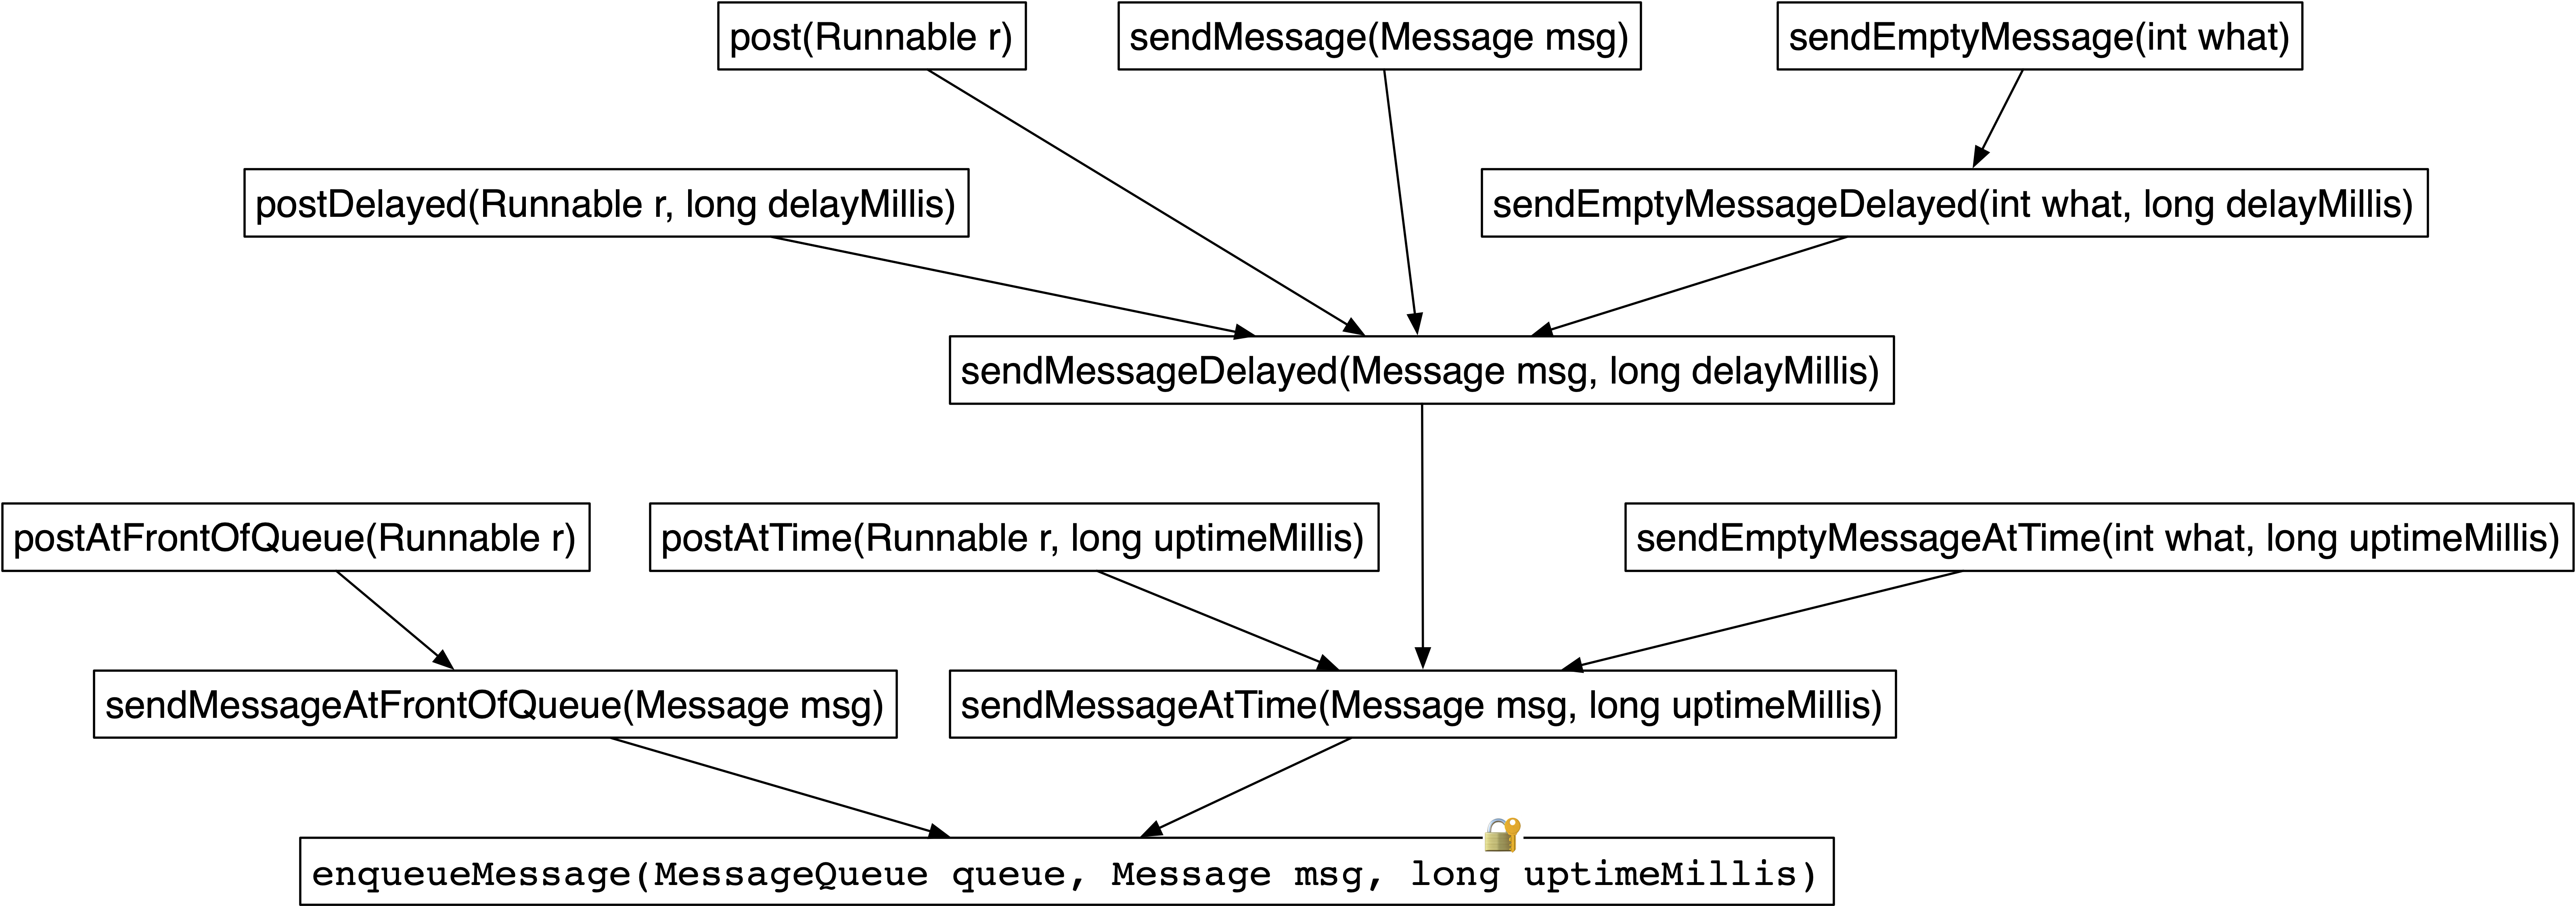
\includegraphics[width=\textwidth]{./Figures/Handler-apis.png}
	\caption{ Handler 各API之间的调用关系}
	\label{fig:handler-apis}
\end{figure*}


除了示例中的调用方式,Android SDK提供的API\cite{HandlerA26:online}还提供多种API(如\autoref{fig:handler-apis}所示),同时支持基于\code{Runnable}的消息调度和基于逻辑代码的消息调度:
%开发人员可以通过\code{post(Runnable)},\code{postAtTime(Runnable,long)},\code{sendMessage(Message)},\code{sendMessageDelayed(Message,long)},\code{sendMessageAtTime(Message,long)}和\code{sendEmptyMessage(int)}等多种API形式实现消息调度。
 通过分析Android系统相关源代码,我们发现上述Handler相关的API关系如\autoref{fig:handler-apis}所示。


Handler机制主要由Handler、Looper、MessageQueue、Message等若干部分共同构成。
%\begin{enumerate}
%		\setlength{\itemsep}{-5pt}
%\item
 Message是多线程交互的核心载体;
%无论开发人员以何种形式调用了Handler发送消息,相关的参数最后均会被封装到Message对象中。
考虑到移动设备的硬件限制以及Message使用的频繁性,Android系统通过对象池对Message对象进行管理。
%\item 
MessageQueue是一个双端队列,存放所有待处理的Message对象。
%开发人员可以根据具体业务场景在消息队列的头部、尾部或者适当位置插入消息队列。
%\item 
Looper负责消息的分发。
%一个线程最多只允许只有一个Looper对象,他只能绑定一个与之对应的MessageQueue;
%其中最为常见的就是位于主线程的MainLooper,它主要负责Android系统的日常调度(例如Activity的生命周期、控件的点击事件响应等)。
%\item
作为消息的发送者和消费者,Handler负责将消息发送到对应的MessageQueue中以及消费来自Looper分发下来的Message。
%在一个应用中,Handler可以存在多个对象,一个Handler对象也可以同时扮演生产者和消费者两个角色。
%\end{enumerate}
Handler机制中各组成部分的相互关系如\autoref{fig:handler-framework}所示。
当用户要通过Handler传递消息时,用户将调用系统提供的Handler API,
该API会将通过分发\code{Handler.enqueueMessage(MessageQueue, Message, long)}将消息投递到消息队列MessageQueue中;
当Looper从MessageQueue中读取该Message对象,分发给对应的Handler对象;
最终,Handler对象通过方法\code{Handler.dispatchMessage(Message)}调用方法\code{Handler.handleMessage(Message)},按照Message对象进行业务逻辑处理。
\begin{figure*}[!ht]
	\centering
	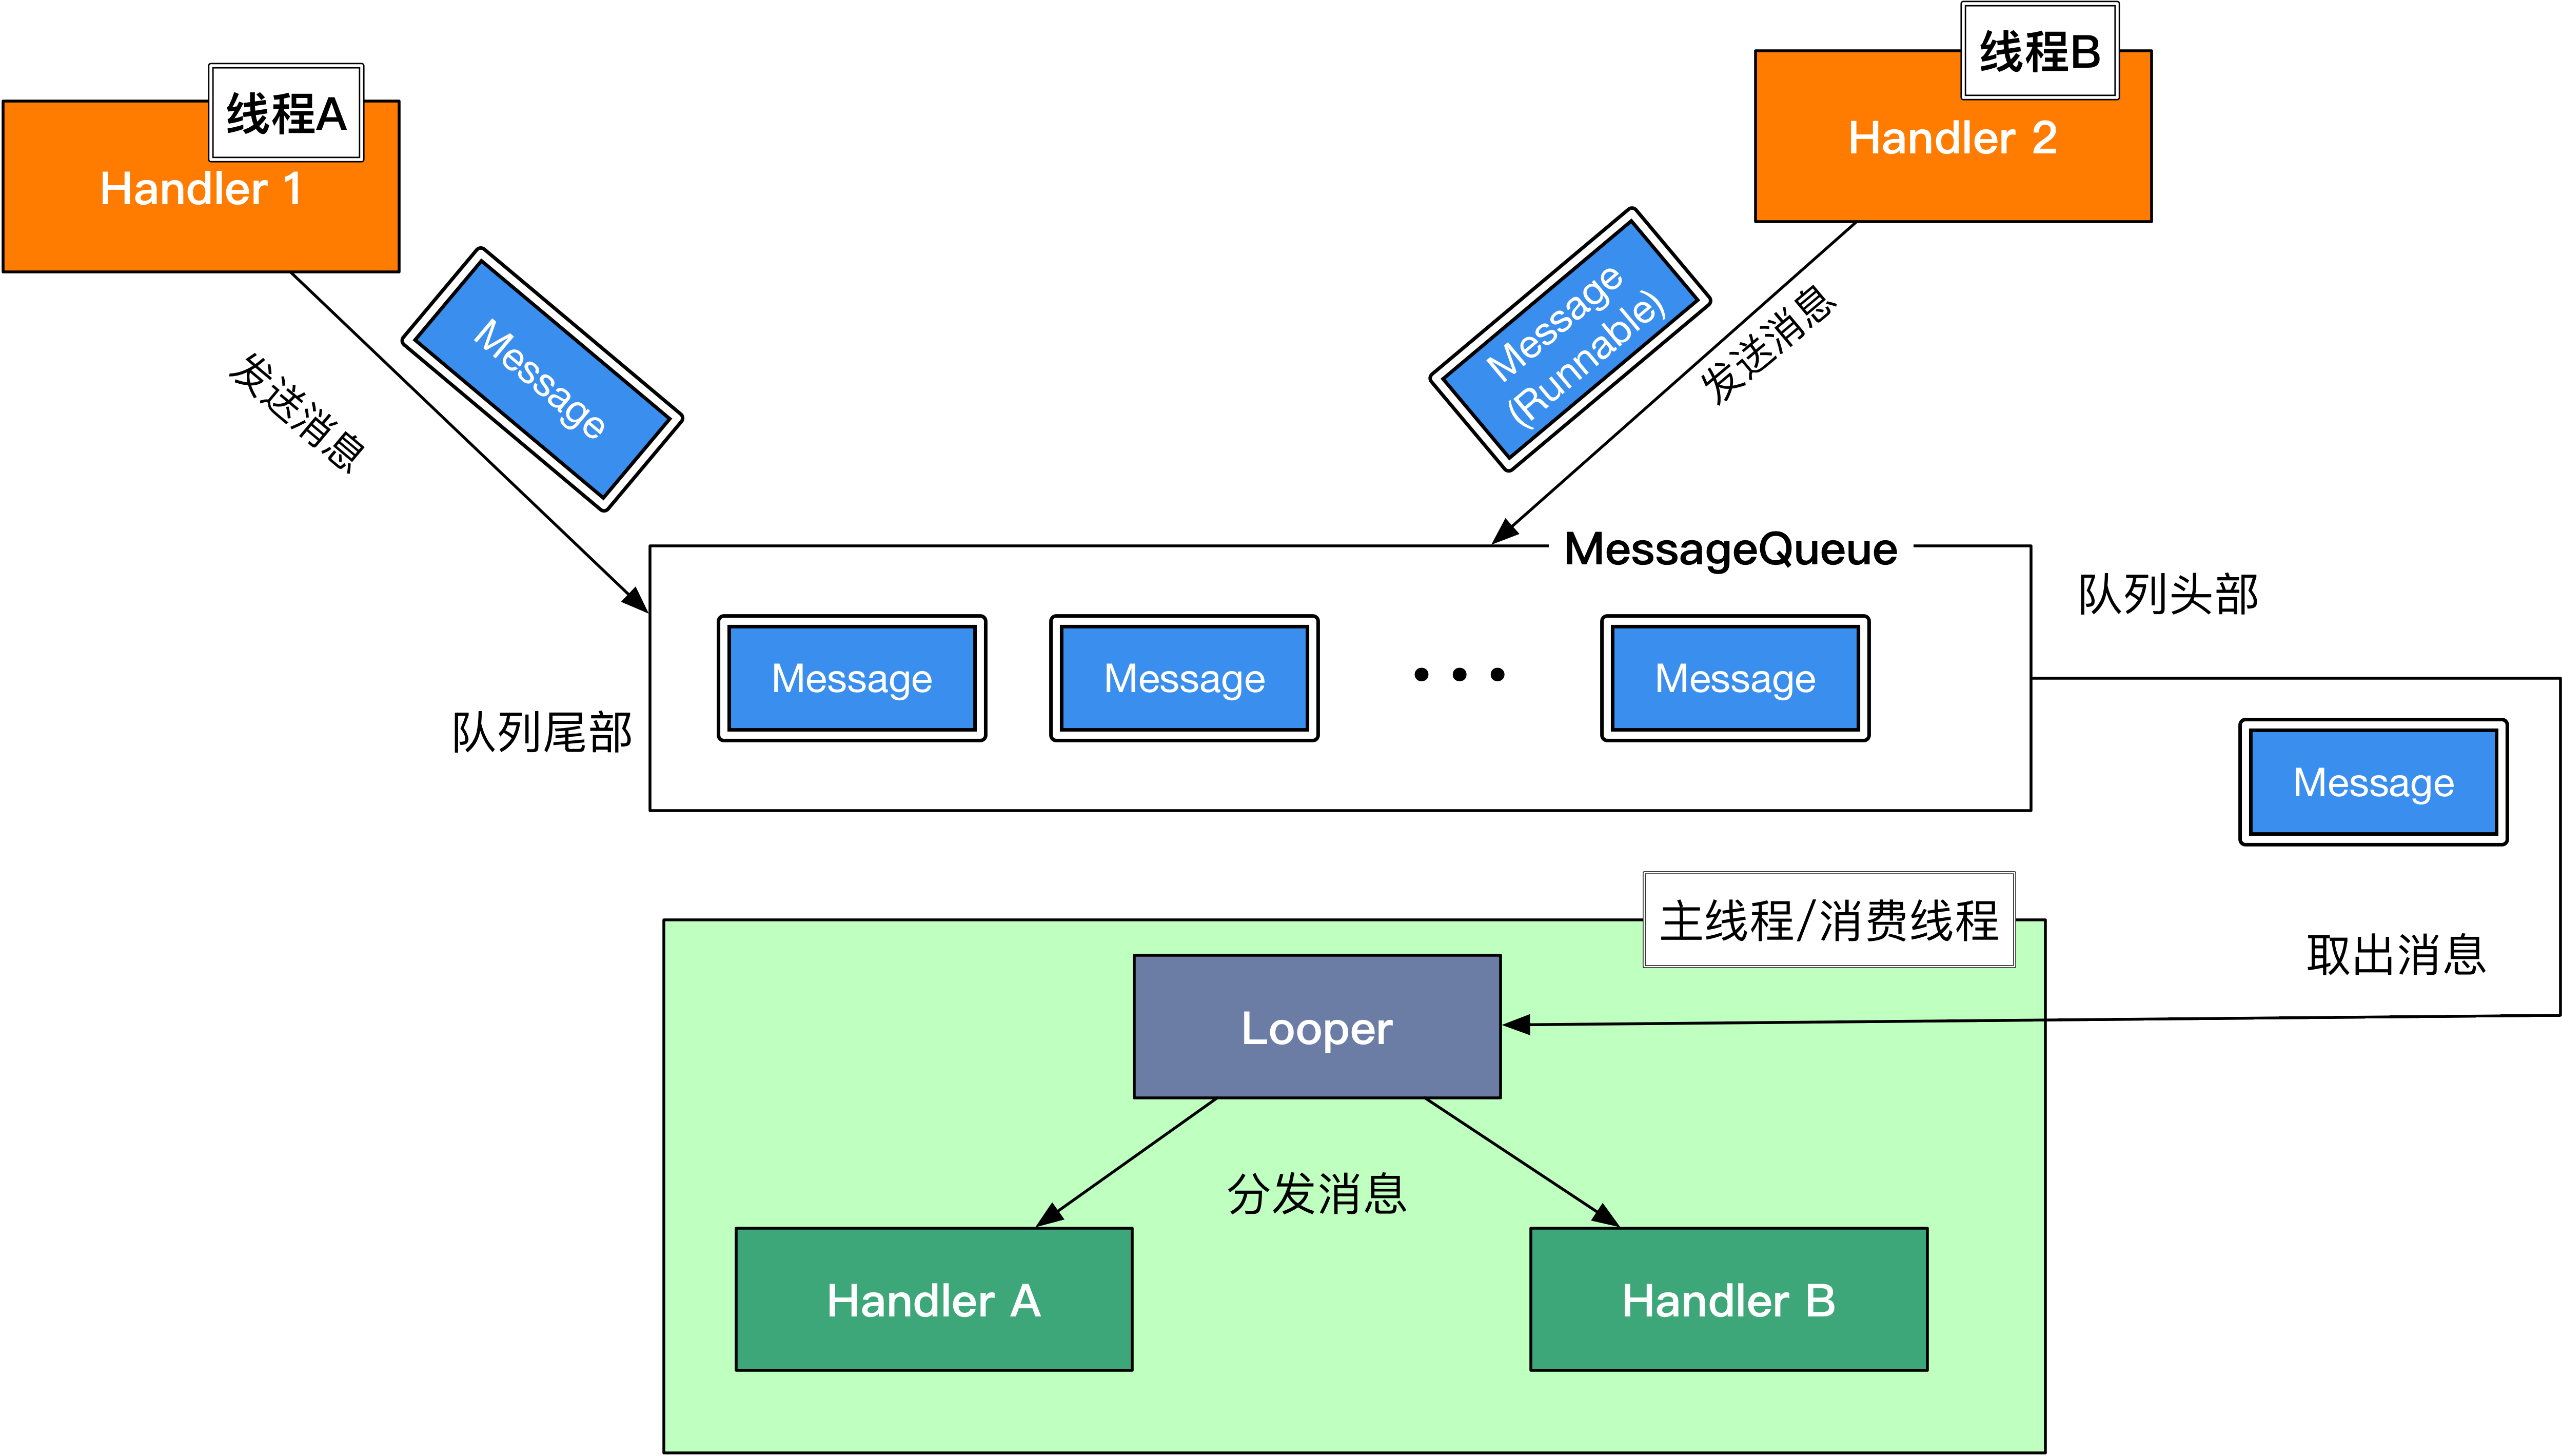
\includegraphics[width=0.8\textwidth]{./Figures/Handler-framework.png}
	\caption{ Handler机制中各组成部分的相互关系}
	\label{fig:handler-framework}
\end{figure*}

基于Handler的多线程消息调度,充分利用了Android的事件驱动架构,将业务逻辑抽象出Message对象,借助消息队列在线程间传递Message,达到了Android多线程交互的目的。
Handler机制,不仅帮助开发人员实现业务逻辑在主线程和工作线程间的自由转移,而且其灵活的API设计降低应用的设计复杂程度,提升了系统架构的可拓展性。
正因如此,在Android开发过程中,基于Handler消息调度的多线程交互十分常见。


\section{本章总结}

本章主要介绍了Android系统的相关背景知识,较为详细的阐述了Android的系统结构,详细介绍了Android四大组件之一的Activity生命周期。
同时,本章还介绍了基于Runnable/Thread、Handler消息调度两种不同的多线程交互方式,详细地分析了Handler的运行机制,为下文基于函数调用图的多线程触发关系生成做了铺垫。
%最后,本章还介绍了系统在实现上可能遇到的困难。
